%====================================================
%  Dark Energy / Late-Time Cosmology Template
%====================================================

\documentclass[
    aps,
    prd,
    twocolumn,
    nofootinbib,
    floatfix,
    superscriptaddress
]{revtex4-2}

%----------------------------------------------------
% Encoding & Fonts
%----------------------------------------------------
\usepackage[T1]{fontenc}
\usepackage[utf8]{inputenc}
\usepackage{lmodern}

%----------------------------------------------------
% Mathematics
%----------------------------------------------------
\usepackage{amsmath, amssymb, amsfonts}
\usepackage{mathtools}
\usepackage{physics}
\usepackage{bm}

%----------------------------------------------------
% Figures & Tables
%----------------------------------------------------
\usepackage{graphicx}
\usepackage{booktabs}
\usepackage{array}

%----------------------------------------------------
% Typography
%----------------------------------------------------
\usepackage{microtype}
\usepackage{enumitem}
\setlist{nosep}

%----------------------------------------------------
% Hyperlinks
%----------------------------------------------------
\usepackage[
    colorlinks=true,
    linkcolor=blue,
    citecolor=blue,
    urlcolor=blue
]{hyperref}

%----------------------------------------------------
% Dark Energy & Cosmology Macros
%----------------------------------------------------

% Omegas
\newcommand{\Om}{\Omega_{\mathrm{m}}}
\newcommand{\Ol}{\Omega_\Lambda}

% Energies
\newcommand{\Ep}{E_\mathrm{peak}}
\newcommand{\Ei}{E_\mathrm{iso}}

%----------------------------------------------------
% Title Information
%----------------------------------------------------
\begin{document}
\title{Cosmological Parameter Inference with Amati GRB relation}

\author{Joan Alcaide-Núñez}
\author{Giancarlo Ghirlanda\thanks{supervisor}}
\author{Om Sharan Salafia\thanks{supervisor}}
\affiliation{Osservatorio Astronomico di Brera (OAB-INAF), Merate, Italy}

\date{\today}

\maketitle

%----------------------------------------------------
% Abstract
%----------------------------------------------------
\begin{abstract}
Should I include the SGRB fits when the results are ready? Should I include the results from the $\chi^2$-volume for H0OmOL?
\end{abstract}

%----------------------------------------------------
% Document
%----------------------------------------------------

% \tableofcontents
\vspace{1em}

%====================================================
\textit{This document summarizes an independent research project under the scientific guidance of Dr. Giancarlo Ghirlanda and Dr. Om Sharan Salafia. The work is exploratory in the nature and intended as a research report for training purposes and is not a peer-review publication.
}

%====================================================
\section{Introduction}
%====================================================

The accelerated expansion of the Universe remains on the of the central open problems in modern cosmology. While the standard $\Lambda$CDM model has provided excellent predictions of a range of observations, the physical nature of dark energy and the precise value of the Hubble constant $(H_0)$ continue to be actively discussed. This unexplained tension between early-universe probes and late-time distance ladder measurements motivate the exploration of complementary and independent probes.

Gamma-ray bursts (GRBs) are among the most luminous transient phenomena in the universe and are detectable over a broad redshift range $(3\lesssim z \lesssim 8)$, extending well beyond that of Type Ia Supernovae (SNe Ia) and any other standard candle. Their luminosities make them appealing candidates for probing distances at high redshift independent from other standard candles relying on empirical correlations between observable properties. While such correlations have been extensively studied (\cite{ghirlanda2006}), their physical origin, intrinsic scatter, and susceptibility to selection effects remain subjects of ongoing research.

In parallel, gravitational-wave (GW) observations have opened a new avenue for cosmology \cite{mastrogiovanni2024}. Compact binary mergers with electromagnetic counterparts provide direct measurements of luminosity distance totally independent from any other methods. Although the current number of observed multi-messenger events is limited to one \cite{ligocollaboration2017}, coming observation campaigns \cite{salafia2025} and future GW detectors, such as Einstein Telescope or Cosmic Explorer, are expected to increase the sample, making standard sirens a promising tool for precision cosmology.

The aim of this project is to explore, within a much simplified framework, the use of GRB empirical relations as cosmological probes and examine the potential of GW joint observations for the same purpose. To this end, ($\Omega_m, \Omega_\Lambda, H_0)$ are inferred by fitting the $E_\text{peak}-E_\text{iso}$ empirical relation and a simulation population of binary neutron star (BNS) mergers using a $\chi^2$ minimization approach. 

This report is structure as follows: section \ref{sec:methodology} defines the cosmological framework and the fitting process for both the GRB relation and the GW Hubble diagram. Section \ref{sec:data} describes the used datasets used in this report, leading to the results in section \ref{sec:results}. Finally, in section \ref{sec:discussion} we discuss the limitations and room for improvement of this basic analysis.


%----------------------------------------------------
% Methodology
%----------------------------------------------------

\section{Methodoogy}\label{sec:methodology}

\subsection{Cosmological Framework}

Throughout this work, we assume a flat $\Lambda$CDM cosmological model $(\Omega_k=0)$, characterized by the Hubble constant $H_0$ and the density parameters of matter $\Omega_m$ and dark energy $\Omega_\Lambda$, and assume the contribution of radiation is negligible $(\Omega_r = 0)$. Under this assumptions the luminosity distance is given by:
$$\label{eq:dl}
d_L (z; H_0, \Omega_m, \Omega_\Lambda) = (1+z) \frac{c}{H_0}\int_0^z\frac{dz^\prime}{\sqrt{\Omega_m (1+z^\prime)^3+\Omega_\Lambda}}
$$
which is evaluated numerically using standard routines from the \verb|astropy.cosmology| library.

\subsection{GRB Empirical Relation}

The first part of the analysis is based on the empirical correlation between the rest-frame peak energy $E_\text{peak}$ and the isotropic equivalent energy $E_\text{peak}$, commonly referred to as the Amati relation \cite{ghirlanda2006}. In logarithmic form, this relation can be written as
$$
\log_{10} E_\text{peak} = a \log_{10} E_\text{iso}
$$
where $a$ and $b$ are the free parameters describing the slope and normalisation of the correlation respectively. The isotropic energy depends explicitly on the assumed cosmology through luminosity distance:
$$
E_\text{iso} = 4\pi d_L(z) \mathcal{F}/(1+z)
$$

where $\mathcal{F}$ is the observed fluence. Due to this dependecy, the parameters of the $E_\text{peak} - E_\text{iso}$ relation and its goodness of fit vary across the cosmological parameter space $(\Omega_m, \Omega_\Lambda, H_0)$.

\subsection{Parameter Estimation via $\chi^2$ Minimzation}

The circularity problem is that in order to know $E_\text{peak}$ and fit the correlation wee need to assume a cosmology, since $E_\text{peak} \propto d_L$. One of the solutions to this issue in the literature (\cite{ghirlanda2008}) is to fit the GRB correlation for all possible cosmologies and building a $\chi^2(\Omega_m, \Omega_\Lambda, H_0)$ space. Then, the cosmology with minimum $\chi^2$ is assumed to be the 'best' cosmology. For a given cosmology choice, the GRB correlation parameters are determined by minimising the $\chi^2$ defined as
$$
\chi^2 = \sum_i \frac{\left[\log_{10}E_\text{peak,i}-(a\log_{10} E_\text{iso,i}+b\right])}{\sigma_{\log E_\text{peak,i}}^2 + \sigma_\text{extra}^2}
$$
where $\sigma_{\log E_\text{peak}}$ denotes the uncertainty for $\log_{10} E_\text{peak}$ and $\sigma_\text{extra}$ is a correlation intrinsic scatter term introduced to account for scatter larger than the measurement uncertainty itself. During the analysis this was set to $\sigma_\text{extra} = \log_{10} (1.3) \approx 0.114$ and held fixed throughout the analysis. By minizing the $\chi2$ fit of the parameters we obtain the $E_\text{peak}-E_\text{iso}$ relation and the parameter space for that cosmology. The location of the minimum and ultimately the $\chi^2$ contours, which with another $\chi^2$ minimization return the 'best' cosmology.

\subsection{Gravitational-Wave Standard Sirens}

In addition to GRB-based constraints, gravitational-wave standard sirens can be used to provide an independent probe of cosmology. The strain of a gravitational wave is inversely proportional to the luminosity distance of the source, with a certain amount of degeneracy due to the system's plane angle. When a gravitational-wave signal is associated with an electromagnetic counterpart, and therefore a host galaxy, the redshift of the source can be measured directly. Then a luminosity-distance-redshift relation (Hubble diagram) can be computed to infer cosmology with reliance on the cosmic ladder.

Due to the limited number of observed multi-messenger events to date, in order to illustrate the complementarity of the gravitational-wave and and GRB-based cosmology inference, a simulated population of binary neutron star (BNS) mergers is employed. This dataset provides redshift and luminosity distance measurements, which are fitted using equation \ref{eq:dl}. Cosmological constraints are then constructed via the Hubble diagram following
$$
\chi^2 = \frac{1}{\mathcal{N}} \sum_i \frac{\left[d_L(\text{data}) - d_L (z; \Omega_m, \Omega_\Lambda, H_0)\right]^2}{\sigma_{d_L}^2}
$$

where $\mathcal{N} = N-n$ are the degrees of freedom, computed from the number of data points $N$ and the number of fitting parameters $(n=3)$.

\subsection{Combined Constraints}

Finnally, the GRB-based and GW-based $\chi^2$ volumes are combined by summing them, assuming statistical independence between the two probes. The resulting joint contraint illustrates the complementarity of electromagnetic and GW observations in constraining cosmological parameters. May the reader be remembered that while GRB data is real, GW data stem from simulations.

\section{Data and Assumptions}

The data for the GRB observations was obtained from \cite{ghiarlanda2008}, which presents a literature summary (1997-2005) of prompt emission energetic parameters for GRBs with measured redshift. All the necessary data for the analysis ($E_\text{peak}, E_\text{iso}$ and $z$ was extracted from there. The redshift range of the samples is $0.125<z<4.9$. From the original table 2 sources were excluded from this analysis due to their exceptionally low $E_\text{peak}$, an order of magnitude smaller than the rest of the entries. For this work, potential effects such as redshift evolution or selection biases are assumed to be negligible and that the authors originally computed $E_\text{peak}$ from the observations assuming the standard cosmology $\Omega_\Lambda = 0.7 = 1 \Omega_m, \Omega_\text{rad} = \Omega_k = 0$.

For the GW data, the simulations results from \cite{colombo2025}, who simulates $10^4$ BNS merger events including the appearance of kilonovae and GRBs and their properties. From this dataset we only use the $d_L$ and $z$ for GW events and $E_\text{peak}$, $E_\text{iso}$ and $z$ for the counterpart GRB event. The issue appeared that parameter fits are not meaningful with $10^4$ parameter points. To solve this, the sample size is reduced to the first $10^3$ data points in the dataset. The redshift range is approximatey up to $z\sim2$, and we also assume that this data does not introduce any effects such as redshift evolution or selection bias. For all the data points we set a fixed $d_L$ uncertainty of $\sigma_{d_L} = 0.1 d_L$.

\section{Results}

\subsection{Constraints from GRB Relations}

Using the methodology described before, the correlation was fitted across the $(\Omega_m, \Omega_\Lambda, H_0)$ parameter space. For each cosmology the $E_\text{peak}-E_\text{iso}$ correlation was fitted through $\chi^2$ minimization, which was recorded as the cosmology's goodness of fit, building a volume which identifies the preferred region with a minimum at

$$
\begin{cases}
	H_0 = 61.25 \\
	\Omega_m = 0.1667 \\
	\Omega_\Lambda = 0.9167
\end{cases}
$$

\begin{figure}
	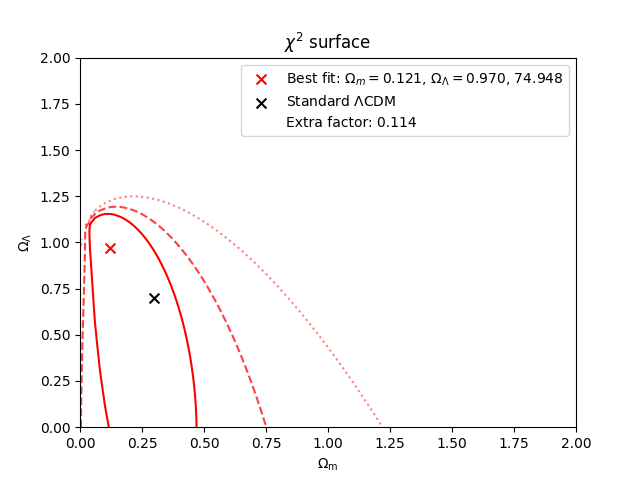
\includegraphics[width=0.8\linewidth]{GRB_surface.png}
	\caption{This is the caption}
\end{figure}

corresponding with a value $\chi^2 = 74.95$. F

Using the methodology described before, the correlation was fitted across the parameter space. The minimum $\chi^2$ is given for the GRB data:

$$
\begin{cases}
	H_0 = 61.25 \\
	\Omega_m = 0.1667 \\
	\Omega_\Lambda = 0.9167
\end{cases}
$$

and for the GW data:

$$
\begin{cases}
	H_0 = 67.3469\\
	\Omega_m = 0.2939 \\
	\Omega_\Lambda = 0.6429
\end{cases}
$$

\subsection{Constraints from GRB Relations}

\section{Discussion}



%----------------------------------------------------
% Acknowledgments
%----------------------------------------------------

%\begin{acknowledgments}
%\end{acknowledgments}

%----------------------------------------------------
% Bibliography
%----------------------------------------------------
\bibliographystyle{apsrev4-2}
\bibliography{references}

\end{document}
